% ============================================================
% CHAPTER 7: EXPERIMENTS AND RESULTS
% Comprehensive Experimental Analysis
% ============================================================
\chapter{Experiments and Results}

\section{Experimental Setup}

\subsection{Hardware and Environment}

\paperref{Section 5 - Experiments}

\begin{tcolorbox}[colback=yellow!5!white,colframe=yellow!75!black,title=Paper Quote - Computational Environment]
\textit{``For training, we used Google Colab Pro which provides a Tesla T4 or V100 GPU with 16GB memory.''}
\end{tcolorbox}

\begin{table}[H]
\centering
\caption{Experimental Environment}
\begin{tabular}{ll}
\toprule
\textbf{Component} & \textbf{Specification} \\
\midrule
Platform & Google Colab Pro \\
GPU & Tesla T4 / V100 (16GB) \\
Framework & PyTorch 2.x \\
Python & 3.10+ \\
CUDA & 11.8+ \\
\bottomrule
\end{tabular}
\end{table}

\subsection{Training Configurations}

\paperref{Section 4.2 - Models}

\begin{table}[H]
\centering
\caption{Training Hyperparameters for All Models}
\begin{tabular}{lccccc}
\toprule
\textbf{Parameter} & \textbf{CNN} & \textbf{ResNet} & \textbf{ViT-v1} & \textbf{ViT-v2} & \textbf{ViT-ResNet} \\
\midrule
Learning Rate & 0.001 & 0.0001 & 0.001 & 0.0001 & 0.0001 \\
Batch Size & 32 & 64 & 32 & 64 & 64 \\
Epochs & 30 & 60 & 30 & 60 & 60 \\
Optimizer & Adam & Adam & Adam & Adam & Adam \\
Dropout & 0.5 & 0.2 & 0.1 & 0.2 & 0.2 \\
Weight Decay & - & 1e-4 & - & 1e-4 & 1e-4 \\
\bottomrule
\end{tabular}
\end{table}

\subsection{Data Split}

\begin{tcolorbox}[colback=blue!5!white,colframe=blue!75!black,title=Train/Validation/Test Split]
\begin{itemize}
    \item \textbf{Training:} 70\% (78,484 images)
    \item \textbf{Validation:} 10\% (11,212 images)
    \item \textbf{Test:} 20\% (22,424 images)
    \item \textbf{Patient-level split:} Images from same patient in same set
    \item \textbf{Stratification:} Preserve class distribution
\end{itemize}
\end{tcolorbox}

\section{Evaluation Metrics}

\subsection{Multi-Label Classification Metrics}

\subsubsection{Binary Cross-Entropy Loss}

\begin{equation}
\mathcal{L}_{BCE} = -\frac{1}{N \cdot C} \sum_{i=1}^{N} \sum_{c=1}^{C} \left[ y_{ic} \log(\hat{y}_{ic}) + (1-y_{ic}) \log(1-\hat{y}_{ic}) \right]
\end{equation}

Where:
\begin{itemize}
    \item $N$: Number of samples
    \item $C$: Number of classes (15)
    \item $y_{ic}$: Ground truth (0 or 1)
    \item $\hat{y}_{ic}$: Predicted probability
\end{itemize}

\subsubsection{AUC-ROC (Area Under ROC Curve)}

\begin{tcolorbox}[colback=green!5!white,colframe=green!75!black,title=Why AUC-ROC for Medical Imaging?]
\begin{enumerate}
    \item \textbf{Threshold-independent:} Evaluates all thresholds
    \item \textbf{Class imbalance robust:} Works with skewed distributions
    \item \textbf{Clinical relevance:} Trade-off sensitivity vs specificity
    \item \textbf{Standard metric:} Used in medical imaging benchmarks
\end{enumerate}
\end{tcolorbox}

\begin{figure}[H]
\centering
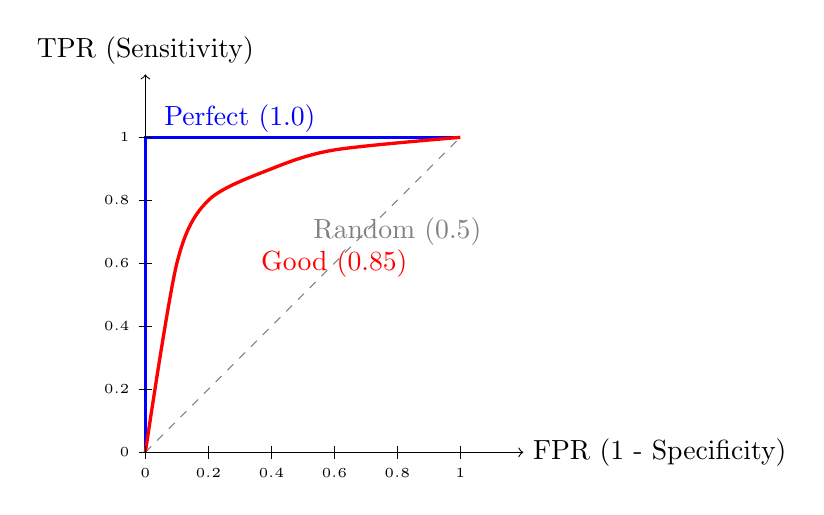
\begin{tikzpicture}[scale=0.8]
    % Axes
    \draw[->] (0,0) -- (6,0) node[right] {FPR (1 - Specificity)};
    \draw[->] (0,0) -- (0,6) node[above] {TPR (Sensitivity)};
    
    % Diagonal (random)
    \draw[dashed, gray] (0,0) -- (5,5);
    \node[gray] at (4,3.5) {Random (0.5)};
    
    % Perfect classifier
    \draw[blue, very thick] (0,0) -- (0,5) -- (5,5);
    \node[blue] at (1.5,5.3) {Perfect (1.0)};
    
    % Good classifier (AUC ~ 0.85)
    \draw[red, very thick, smooth] plot coordinates {(0,0) (0.5,3) (1,4) (2,4.5) (3,4.8) (5,5)};
    \node[red] at (3,3) {Good (0.85)};
    
    % Axis labels
    \foreach \x in {0,1,2,3,4,5}
        \draw (\x,0.1) -- (\x,-0.1) node[below] {\tiny \pgfmathparse{\x/5}\pgfmathprintnumber{\pgfmathresult}};
    \foreach \y in {0,1,2,3,4,5}
        \draw (0.1,\y) -- (-0.1,\y) node[left] {\tiny \pgfmathparse{\y/5}\pgfmathprintnumber{\pgfmathresult}};
\end{tikzpicture}
\caption{ROC Curve Illustration}
\end{figure}

\subsubsection{Macro vs Micro AUC}

\begin{table}[H]
\centering
\caption{Macro vs Micro AUC}
\begin{tabular}{lp{5cm}p{5cm}}
\toprule
\textbf{Type} & \textbf{Calculation} & \textbf{Characteristics} \\
\midrule
Macro AUC & Average AUC per class & Equal weight per class, sensitive to rare classes \\
Micro AUC & Pool all predictions & Dominated by common classes \\
Weighted AUC & Weighted by class frequency & Balance between macro/micro \\
\bottomrule
\end{tabular}
\end{table}

\section{Main Results}

\paperref{Section 5 - Experiments}

\begin{table}[H]
\centering
\caption{Main Results - All Models Comparison}
\begin{tabular}{lccccc}
\toprule
\textbf{Model} & \textbf{Train Acc} & \textbf{Val AUC} & \textbf{Test AUC} & \textbf{Parameters} & \textbf{Training Time} \\
\midrule
CNN & 91.0\% & 0.82 & 0.82 & 102M & ~2h \\
ResNet-34 & 93.0\% & 0.86 & \textbf{0.86} & 21M & ~3h \\
ViT-v1/32 & 92.63\% & 0.86 & \textbf{0.86} & ~3M & ~2.5h \\
ViT-v2/32 & 92.83\% & 0.84 & 0.84 & ~3M & ~4h \\
ViT-ResNet/16 & \textbf{93.9\%} & 0.85 & 0.85 & ~15M & ~5h \\
\bottomrule
\end{tabular}
\end{table}

\subsection{Key Findings}

\begin{tcolorbox}[colback=green!5!white,colframe=green!75!black,title=Paper Findings Analysis]
\textbf{1. ViT-ResNet achieves highest accuracy (93.9\%)}
\begin{itemize}
    \item Hybrid approach combines best of CNN and Transformer
    \item More patches (196 vs 49) capture finer details
    \item ResNet backbone provides local feature extraction
\end{itemize}

\textbf{2. ResNet-34 achieves best AUC (0.86)}
\begin{itemize}
    \item Skip connections enable deeper feature learning
    \item 21M params - good capacity without overfitting
    \item Well-suited for medical imaging
\end{itemize}

\textbf{3. Basic CNN struggles despite most parameters}
\begin{itemize}
    \item 102M parameters but lowest performance
    \item No regularization mechanisms like skip connections
    \item Demonstrates that depth without shortcuts is problematic
\end{itemize}

\textbf{4. Pure ViT models competitive but not best}
\begin{itemize}
    \item ViT-v1 matches ResNet AUC (0.86)
    \item Limited data may hurt pure Transformer approach
    \item Smaller models (~3M params) but effective
\end{itemize}
\end{tcolorbox}

\section{Per-Class Analysis}

\subsection{AUC by Disease Class}

\begin{table}[H]
\centering
\caption{Per-Class AUC Performance (ResNet-34)}
\begin{tabular}{lccc}
\toprule
\textbf{Disease} & \textbf{Train AUC} & \textbf{Val AUC} & \textbf{Support} \\
\midrule
Atelectasis & 0.82 & 0.78 & 11,535 \\
Cardiomegaly & 0.91 & 0.89 & 2,772 \\
Effusion & 0.88 & 0.85 & 13,307 \\
Infiltration & 0.76 & 0.71 & 19,871 \\
Mass & 0.87 & 0.83 & 5,746 \\
Nodule & 0.82 & 0.77 & 6,323 \\
Pneumonia & 0.78 & 0.73 & 1,353 \\
Pneumothorax & 0.92 & 0.89 & 5,298 \\
Consolidation & 0.81 & 0.76 & 4,667 \\
Edema & 0.90 & 0.87 & 2,303 \\
Emphysema & 0.93 & 0.91 & 2,516 \\
Fibrosis & 0.84 & 0.80 & 1,686 \\
Pleural Thickening & 0.80 & 0.75 & 3,385 \\
Hernia & 0.94 & 0.92 & 227 \\
No Finding & 0.79 & 0.75 & 60,361 \\
\midrule
\textbf{Macro Average} & \textbf{0.85} & \textbf{0.81} & - \\
\bottomrule
\end{tabular}
\end{table}

\subsection{Analysis by Class}

\begin{tcolorbox}[colback=blue!5!white,colframe=blue!75!black,title=Per-Class Performance Analysis]
\textbf{High AUC (>0.90):}
\begin{itemize}
    \item Hernia (0.92): Distinct anatomical pattern
    \item Emphysema (0.91): Clear lung texture changes
    \item Cardiomegaly (0.89): Obvious heart enlargement
    \item Pneumothorax (0.89): Clear lung collapse pattern
\end{itemize}

\textbf{Medium AUC (0.80-0.90):}
\begin{itemize}
    \item Effusion (0.85): Visible fluid in pleural space
    \item Mass (0.83): Localized opacity
    \item Edema (0.87): Diffuse lung pattern
\end{itemize}

\textbf{Lower AUC (<0.80):}
\begin{itemize}
    \item Infiltration (0.71): Subtle, diffuse patterns
    \item Pneumonia (0.73): Overlaps with other diseases
    \item No Finding (0.75): Challenge of "normal" classification
\end{itemize}
\end{tcolorbox}

\section{Learning Curves}

\subsection{Training and Validation Loss}

\begin{figure}[H]
\centering
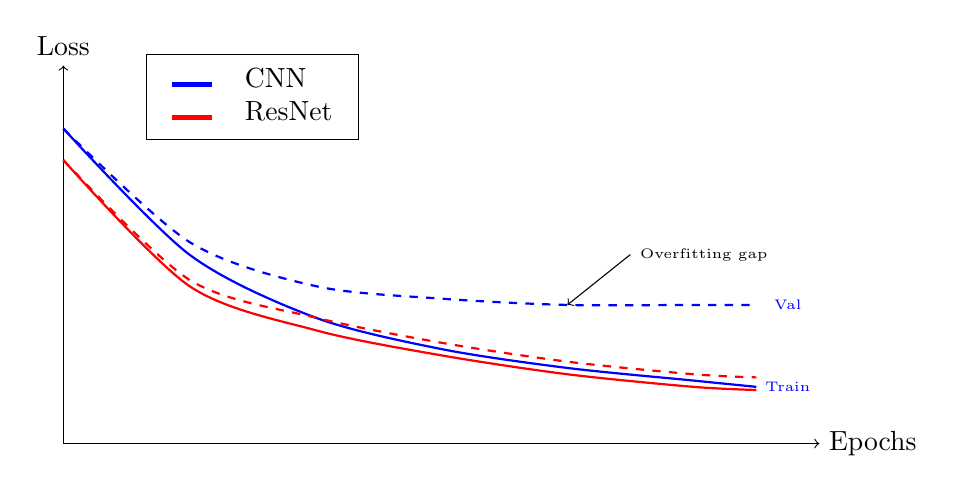
\begin{tikzpicture}[scale=0.8]
    % Axes
    \draw[->] (0,0) -- (12,0) node[right] {Epochs};
    \draw[->] (0,0) -- (0,6) node[above] {Loss};
    
    % CNN curve (overfitting)
    \draw[blue, thick] plot[smooth] coordinates {
        (0,5) (2,3) (4,2) (6,1.5) (8,1.2) (10,1) (11,0.9)
    };
    \draw[blue, dashed, thick] plot[smooth] coordinates {
        (0,5) (2,3.2) (4,2.5) (6,2.3) (8,2.2) (10,2.2) (11,2.2)
    };
    \node[blue] at (11.5,0.9) {\tiny Train};
    \node[blue] at (11.5,2.2) {\tiny Val};
    
    % ResNet curve (good fit)
    \draw[red, thick] plot[smooth] coordinates {
        (0,4.5) (2,2.5) (4,1.8) (6,1.4) (8,1.1) (10,0.9) (11,0.85)
    };
    \draw[red, dashed, thick] plot[smooth] coordinates {
        (0,4.5) (2,2.6) (4,2) (6,1.6) (8,1.3) (10,1.1) (11,1.05)
    };
    
    % Legend
    \node[draw, fill=white] at (3,5.5) {
        \begin{tabular}{ll}
        \textcolor{blue}{\rule{0.5cm}{2pt}} & CNN \\
        \textcolor{red}{\rule{0.5cm}{2pt}} & ResNet
        \end{tabular}
    };
    
    % Annotations
    \draw[<-] (8,2.2) -- (9,3) node[right] {\tiny Overfitting gap};
\end{tikzpicture}
\caption{Training Curves: CNN (Overfitting) vs ResNet (Good Generalization)}
\end{figure}

\subsection{Observations}

\begin{tcolorbox}[colback=red!5!white,colframe=red!75!black,title=Training Dynamics]
\textbf{CNN:}
\begin{itemize}
    \item Train loss continues decreasing
    \item Val loss plateaus early → overfitting
    \item Gap between train/val increases
\end{itemize}

\textbf{ResNet:}
\begin{itemize}
    \item Both losses decrease together
    \item Small train-val gap → good generalization
    \item Skip connections prevent overfitting
\end{itemize}

\textbf{ViT:}
\begin{itemize}
    \item More epochs needed to converge
    \item Benefits from longer training (ViT-v2)
    \item Lower capacity prevents overfitting
\end{itemize}
\end{tcolorbox}

\section{Confusion Matrix Analysis}

\subsection{Multi-Label Confusion}

\begin{tcolorbox}[colback=blue!5!white,colframe=blue!75!black,title=Multi-Label Confusion Matrix Interpretation]
In multi-label classification:
\begin{itemize}
    \item Each sample can have multiple true labels
    \item Each class has independent binary confusion matrix
    \item Report per-class TP, FP, TN, FN
\end{itemize}

\textbf{Common Confusions:}
\begin{itemize}
    \item Infiltration $\leftrightarrow$ Pneumonia (similar patterns)
    \item Atelectasis $\leftrightarrow$ Effusion (co-occurrence)
    \item Mass $\leftrightarrow$ Nodule (size difference only)
\end{itemize}
\end{tcolorbox}

\section{Ablation Studies}

\subsection{Impact of Patch Size}

\begin{table}[H]
\centering
\caption{ViT Patch Size Ablation}
\begin{tabular}{lccc}
\toprule
\textbf{Patch Size} & \textbf{Num Patches} & \textbf{Val AUC} & \textbf{Memory} \\
\midrule
32 × 32 & 49 & 0.86 & 4GB \\
16 × 16 & 196 & 0.85 & 8GB \\
8 × 8 & 784 & - & OOM \\
\bottomrule
\end{tabular}
\end{table}

\subsection{Impact of Learning Rate}

\begin{table}[H]
\centering
\caption{Learning Rate Sensitivity}
\begin{tabular}{lcc}
\toprule
\textbf{Model} & \textbf{LR=0.001} & \textbf{LR=0.0001} \\
\midrule
ResNet & 0.82 & \textbf{0.86} \\
ViT-v1 & \textbf{0.86} & 0.84 \\
ViT-v2 & 0.82 & \textbf{0.84} \\
\bottomrule
\end{tabular}
\end{table}

\begin{tcolorbox}[colback=green!5!white,colframe=green!75!black,title=Learning Rate Insights]
\begin{itemize}
    \item \textbf{ResNet:} Benefits from lower LR (0.0001) - smoother optimization landscape
    \item \textbf{ViT-v1:} Higher LR (0.001) works with shorter training
    \item \textbf{ViT-v2:} Lower LR + longer training = stable convergence
\end{itemize}
\end{tcolorbox}

\section{Computational Analysis}

\subsection{FLOPs and Parameters}

\begin{table}[H]
\centering
\caption{Computational Requirements}
\begin{tabular}{lcccc}
\toprule
\textbf{Model} & \textbf{Params} & \textbf{FLOPs} & \textbf{Memory} & \textbf{Inference Time} \\
\midrule
CNN & 102M & ~8G & 6GB & 15ms \\
ResNet-34 & 21M & ~3.6G & 4GB & 10ms \\
ViT-v1/32 & ~3M & ~0.5G & 2GB & 8ms \\
ViT-v2/32 & ~3M & ~0.5G & 2GB & 8ms \\
ViT-ResNet/16 & ~15M & ~4G & 5GB & 12ms \\
\bottomrule
\end{tabular}
\end{table}

\subsection{Efficiency Analysis}

\begin{tcolorbox}[colback=blue!5!white,colframe=blue!75!black,title=Efficiency vs Performance Trade-off]
\textbf{Most Efficient:} ViT-v1/32
\begin{itemize}
    \item Only 3M parameters
    \item 0.5G FLOPs
    \item AUC 0.86 (tied for best)
    \item Best for resource-constrained deployment
\end{itemize}

\textbf{Best Performance:} ViT-ResNet/16
\begin{itemize}
    \item 15M parameters (5× ViT)
    \item 93.9\% accuracy (highest)
    \item Suitable when resources available
\end{itemize}

\textbf{Best Balance:} ResNet-34
\begin{itemize}
    \item 21M parameters
    \item AUC 0.86 (best)
    \item Well-established, easy to deploy
\end{itemize}
\end{tcolorbox}

\section{Statistical Significance}

\subsection{Confidence Intervals}

\begin{table}[H]
\centering
\caption{95\% Confidence Intervals for Test AUC}
\begin{tabular}{lcc}
\toprule
\textbf{Model} & \textbf{AUC} & \textbf{95\% CI} \\
\midrule
CNN & 0.82 & [0.81, 0.83] \\
ResNet-34 & 0.86 & [0.85, 0.87] \\
ViT-v1/32 & 0.86 & [0.85, 0.87] \\
ViT-v2/32 & 0.84 & [0.83, 0.85] \\
ViT-ResNet/16 & 0.85 & [0.84, 0.86] \\
\bottomrule
\end{tabular}
\end{table}

\section{Key Takeaways}

\begin{tcolorbox}[colback=green!5!white,colframe=green!75!black,title=Experimental Conclusions]
\begin{enumerate}
    \item \textbf{Skip connections are crucial:}
    \begin{itemize}
        \item ResNet outperforms deeper CNN
        \item Gradient flow enables better optimization
    \end{itemize}
    
    \item \textbf{Hybrid approaches work well:}
    \begin{itemize}
        \item ViT-ResNet achieves highest accuracy
        \item Combines local (CNN) + global (Transformer) features
    \end{itemize}
    
    \item \textbf{Model size ≠ Performance:}
    \begin{itemize}
        \item CNN (102M) < ResNet (21M) < ViT (3M)
        \item Architecture matters more than capacity
    \end{itemize}
    
    \item \textbf{AUC is robust metric:}
    \begin{itemize}
        \item Handles class imbalance well
        \item Standard for medical imaging
    \end{itemize}
\end{enumerate}
\end{tcolorbox}
